\documentclass[letterpaper,10pt,titlepage]{article}

% This might mess up formatting
\setlength{\parindent}{0pt}

\usepackage{graphicx}
\usepackage{amssymb}
\usepackage{amsmath}
\usepackage{amsthm}

\usepackage{alltt}
\usepackage{float}
\usepackage{color}
\usepackage{url}
\usepackage{listings}
\usepackage{biblatex}
\usepackage{filecontents}

\usepackage{balance}
\usepackage[TABBOTCAP, tight]{subfigure}
\usepackage{enumitem}
\usepackage{pstricks, pst-node}

\usepackage{geometry}
\geometry{textheight=8.5in, textwidth=6in}

\newcommand{\cred}[1]{{\color{red}#1}}
\newcommand{\cblue}[1]{{\color{blue}#1}}

\usepackage{hyperref}
\usepackage{graphicx}
\usepackage{pgfgantt}

\lstdefinestyle{customc}{
  belowcaptionskip=1\baselineskip,
  breaklines=true,
  frame=L,
  xleftmargin=\parindent,
  language=C,
  showstringspaces=false,
  basicstyle=\footnotesize\ttfamily,
  keywordstyle=\bfseries\color{green!40!black},
  commentstyle=\itshape\color{purple!40!black},
  identifierstyle=\color{blue},
  stringstyle=\color{orange},
}

\def\name{Brandon Lee}

%pull in the necessary preamble matter for pygments output
% \usepackage{fancyvrb}
\usepackage{color}
\usepackage[latin1]{inputenc}


\makeatletter
\def\PY@reset{\let\PY@it=\relax \let\PY@bf=\relax%
    \let\PY@ul=\relax \let\PY@tc=\relax%
    \let\PY@bc=\relax \let\PY@ff=\relax}
\def\PY@tok#1{\csname PY@tok@#1\endcsname}
\def\PY@toks#1+{\ifx\relax#1\empty\else%
    \PY@tok{#1}\expandafter\PY@toks\fi}
\def\PY@do#1{\PY@bc{\PY@tc{\PY@ul{%
    \PY@it{\PY@bf{\PY@ff{#1}}}}}}}
\def\PY#1#2{\PY@reset\PY@toks#1+\relax+\PY@do{#2}}

\expandafter\def\csname PY@tok@gd\endcsname{\def\PY@tc##1{\textcolor[rgb]{0.63,0.00,0.00}{##1}}}
\expandafter\def\csname PY@tok@gu\endcsname{\let\PY@bf=\textbf\def\PY@tc##1{\textcolor[rgb]{0.50,0.00,0.50}{##1}}}
\expandafter\def\csname PY@tok@gt\endcsname{\def\PY@tc##1{\textcolor[rgb]{0.00,0.25,0.82}{##1}}}
\expandafter\def\csname PY@tok@gs\endcsname{\let\PY@bf=\textbf}
\expandafter\def\csname PY@tok@gr\endcsname{\def\PY@tc##1{\textcolor[rgb]{1.00,0.00,0.00}{##1}}}
\expandafter\def\csname PY@tok@cm\endcsname{\let\PY@it=\textit\def\PY@tc##1{\textcolor[rgb]{0.25,0.50,0.50}{##1}}}
\expandafter\def\csname PY@tok@vg\endcsname{\def\PY@tc##1{\textcolor[rgb]{0.10,0.09,0.49}{##1}}}
\expandafter\def\csname PY@tok@m\endcsname{\def\PY@tc##1{\textcolor[rgb]{0.40,0.40,0.40}{##1}}}
\expandafter\def\csname PY@tok@mh\endcsname{\def\PY@tc##1{\textcolor[rgb]{0.40,0.40,0.40}{##1}}}
\expandafter\def\csname PY@tok@go\endcsname{\def\PY@tc##1{\textcolor[rgb]{0.50,0.50,0.50}{##1}}}
\expandafter\def\csname PY@tok@ge\endcsname{\let\PY@it=\textit}
\expandafter\def\csname PY@tok@vc\endcsname{\def\PY@tc##1{\textcolor[rgb]{0.10,0.09,0.49}{##1}}}
\expandafter\def\csname PY@tok@il\endcsname{\def\PY@tc##1{\textcolor[rgb]{0.40,0.40,0.40}{##1}}}
\expandafter\def\csname PY@tok@cs\endcsname{\let\PY@it=\textit\def\PY@tc##1{\textcolor[rgb]{0.25,0.50,0.50}{##1}}}
\expandafter\def\csname PY@tok@cp\endcsname{\def\PY@tc##1{\textcolor[rgb]{0.74,0.48,0.00}{##1}}}
\expandafter\def\csname PY@tok@gi\endcsname{\def\PY@tc##1{\textcolor[rgb]{0.00,0.63,0.00}{##1}}}
\expandafter\def\csname PY@tok@gh\endcsname{\let\PY@bf=\textbf\def\PY@tc##1{\textcolor[rgb]{0.00,0.00,0.50}{##1}}}
\expandafter\def\csname PY@tok@ni\endcsname{\let\PY@bf=\textbf\def\PY@tc##1{\textcolor[rgb]{0.60,0.60,0.60}{##1}}}
\expandafter\def\csname PY@tok@nl\endcsname{\def\PY@tc##1{\textcolor[rgb]{0.63,0.63,0.00}{##1}}}
\expandafter\def\csname PY@tok@nn\endcsname{\let\PY@bf=\textbf\def\PY@tc##1{\textcolor[rgb]{0.00,0.00,1.00}{##1}}}
\expandafter\def\csname PY@tok@no\endcsname{\def\PY@tc##1{\textcolor[rgb]{0.53,0.00,0.00}{##1}}}
\expandafter\def\csname PY@tok@na\endcsname{\def\PY@tc##1{\textcolor[rgb]{0.49,0.56,0.16}{##1}}}
\expandafter\def\csname PY@tok@nb\endcsname{\def\PY@tc##1{\textcolor[rgb]{0.00,0.50,0.00}{##1}}}
\expandafter\def\csname PY@tok@nc\endcsname{\let\PY@bf=\textbf\def\PY@tc##1{\textcolor[rgb]{0.00,0.00,1.00}{##1}}}
\expandafter\def\csname PY@tok@nd\endcsname{\def\PY@tc##1{\textcolor[rgb]{0.67,0.13,1.00}{##1}}}
\expandafter\def\csname PY@tok@ne\endcsname{\let\PY@bf=\textbf\def\PY@tc##1{\textcolor[rgb]{0.82,0.25,0.23}{##1}}}
\expandafter\def\csname PY@tok@nf\endcsname{\def\PY@tc##1{\textcolor[rgb]{0.00,0.00,1.00}{##1}}}
\expandafter\def\csname PY@tok@si\endcsname{\let\PY@bf=\textbf\def\PY@tc##1{\textcolor[rgb]{0.73,0.40,0.53}{##1}}}
\expandafter\def\csname PY@tok@s2\endcsname{\def\PY@tc##1{\textcolor[rgb]{0.73,0.13,0.13}{##1}}}
\expandafter\def\csname PY@tok@vi\endcsname{\def\PY@tc##1{\textcolor[rgb]{0.10,0.09,0.49}{##1}}}
\expandafter\def\csname PY@tok@nt\endcsname{\let\PY@bf=\textbf\def\PY@tc##1{\textcolor[rgb]{0.00,0.50,0.00}{##1}}}
\expandafter\def\csname PY@tok@nv\endcsname{\def\PY@tc##1{\textcolor[rgb]{0.10,0.09,0.49}{##1}}}
\expandafter\def\csname PY@tok@s1\endcsname{\def\PY@tc##1{\textcolor[rgb]{0.73,0.13,0.13}{##1}}}
\expandafter\def\csname PY@tok@sh\endcsname{\def\PY@tc##1{\textcolor[rgb]{0.73,0.13,0.13}{##1}}}
\expandafter\def\csname PY@tok@sc\endcsname{\def\PY@tc##1{\textcolor[rgb]{0.73,0.13,0.13}{##1}}}
\expandafter\def\csname PY@tok@sx\endcsname{\def\PY@tc##1{\textcolor[rgb]{0.00,0.50,0.00}{##1}}}
\expandafter\def\csname PY@tok@bp\endcsname{\def\PY@tc##1{\textcolor[rgb]{0.00,0.50,0.00}{##1}}}
\expandafter\def\csname PY@tok@c1\endcsname{\let\PY@it=\textit\def\PY@tc##1{\textcolor[rgb]{0.25,0.50,0.50}{##1}}}
\expandafter\def\csname PY@tok@kc\endcsname{\let\PY@bf=\textbf\def\PY@tc##1{\textcolor[rgb]{0.00,0.50,0.00}{##1}}}
\expandafter\def\csname PY@tok@c\endcsname{\let\PY@it=\textit\def\PY@tc##1{\textcolor[rgb]{0.25,0.50,0.50}{##1}}}
\expandafter\def\csname PY@tok@mf\endcsname{\def\PY@tc##1{\textcolor[rgb]{0.40,0.40,0.40}{##1}}}
\expandafter\def\csname PY@tok@err\endcsname{\def\PY@bc##1{\setlength{\fboxsep}{0pt}\fcolorbox[rgb]{1.00,0.00,0.00}{1,1,1}{\strut ##1}}}
\expandafter\def\csname PY@tok@kd\endcsname{\let\PY@bf=\textbf\def\PY@tc##1{\textcolor[rgb]{0.00,0.50,0.00}{##1}}}
\expandafter\def\csname PY@tok@ss\endcsname{\def\PY@tc##1{\textcolor[rgb]{0.10,0.09,0.49}{##1}}}
\expandafter\def\csname PY@tok@sr\endcsname{\def\PY@tc##1{\textcolor[rgb]{0.73,0.40,0.53}{##1}}}
\expandafter\def\csname PY@tok@mo\endcsname{\def\PY@tc##1{\textcolor[rgb]{0.40,0.40,0.40}{##1}}}
\expandafter\def\csname PY@tok@kn\endcsname{\let\PY@bf=\textbf\def\PY@tc##1{\textcolor[rgb]{0.00,0.50,0.00}{##1}}}
\expandafter\def\csname PY@tok@mi\endcsname{\def\PY@tc##1{\textcolor[rgb]{0.40,0.40,0.40}{##1}}}
\expandafter\def\csname PY@tok@gp\endcsname{\let\PY@bf=\textbf\def\PY@tc##1{\textcolor[rgb]{0.00,0.00,0.50}{##1}}}
\expandafter\def\csname PY@tok@o\endcsname{\def\PY@tc##1{\textcolor[rgb]{0.40,0.40,0.40}{##1}}}
\expandafter\def\csname PY@tok@kr\endcsname{\let\PY@bf=\textbf\def\PY@tc##1{\textcolor[rgb]{0.00,0.50,0.00}{##1}}}
\expandafter\def\csname PY@tok@s\endcsname{\def\PY@tc##1{\textcolor[rgb]{0.73,0.13,0.13}{##1}}}
\expandafter\def\csname PY@tok@kp\endcsname{\def\PY@tc##1{\textcolor[rgb]{0.00,0.50,0.00}{##1}}}
\expandafter\def\csname PY@tok@w\endcsname{\def\PY@tc##1{\textcolor[rgb]{0.73,0.73,0.73}{##1}}}
\expandafter\def\csname PY@tok@kt\endcsname{\def\PY@tc##1{\textcolor[rgb]{0.69,0.00,0.25}{##1}}}
\expandafter\def\csname PY@tok@ow\endcsname{\let\PY@bf=\textbf\def\PY@tc##1{\textcolor[rgb]{0.67,0.13,1.00}{##1}}}
\expandafter\def\csname PY@tok@sb\endcsname{\def\PY@tc##1{\textcolor[rgb]{0.73,0.13,0.13}{##1}}}
\expandafter\def\csname PY@tok@k\endcsname{\let\PY@bf=\textbf\def\PY@tc##1{\textcolor[rgb]{0.00,0.50,0.00}{##1}}}
\expandafter\def\csname PY@tok@se\endcsname{\let\PY@bf=\textbf\def\PY@tc##1{\textcolor[rgb]{0.73,0.40,0.13}{##1}}}
\expandafter\def\csname PY@tok@sd\endcsname{\let\PY@it=\textit\def\PY@tc##1{\textcolor[rgb]{0.73,0.13,0.13}{##1}}}

\def\PYZbs{\char`\\}
\def\PYZus{\char`\_}
\def\PYZob{\char`\{}
\def\PYZcb{\char`\}}
\def\PYZca{\char`\^}
\def\PYZam{\char`\&}
\def\PYZlt{\char`\<}
\def\PYZgt{\char`\>}
\def\PYZsh{\char`\#}
\def\PYZpc{\char`\%}
\def\PYZdl{\char`\$}
\def\PYZti{\char`\~}
% for compatibility with earlier versions
\def\PYZat{@}
\def\PYZlb{[}
\def\PYZrb{]}
\makeatother


%% The following metadata will show up in the PDF properties
\hypersetup{
  colorlinks = true,
  urlcolor = black,
  pdfauthor = {\name},
  pdfkeywords = {CS461 ``Senior Capstone''},
  pdftitle = {CS 461 Design Document},
  pdfsubject = {CS 461 Design Document},
  pdfpagemode = UseNone
}

\begin{document}

\begin{titlepage}
    \begin{center}
        \vspace*{3.5cm}

        \textbf{Design Document}

        \vspace{0.5cm}

        \textbf{Brandon Lee, Rutger Farry, Michael Lee}

        \vspace{0.8cm}

        CS 461\\
        Fall 2016\\
        2 December 2016\\

        \vspace{1cm}

        \textbf{Abstract}\\

        \vspace{0.5cm}

		The purpose of this document is to elaborate the details of the design of our application, C7FIT. The following document will consist of five core parts discussing areas of design in the development of our application including an overview, definitions, conceptual models for software design descriptions, design description information content, and design viewpoints.

        \vfill

    \end{center}
\end{titlepage}

\newpage

\tableofcontents

\newpage

\section{Overview}

\subsection{Scope}
This document will use a level of abstraction that is brief enough for an interested reader to absorb, but in-depth enough for a team of experienced programmers to implement. We cover all aspects of the application architecture, as well as some choices we've made to standardize our development practices and development environment.

\subsection{Purpose}
The intent of this paper is to document the architectural and design choices the C7Fit team has made in designing the C7FIT iOS application. As the app has not been implemented in code  yet, this version of the document should not be considered as a guidebook to the final software implementation. The main purpose is to codify our intent as a reference when we begin implementing the software, and we intend to reflect these intentions in our software as closely as possible / reasonable. This document is subject to change as we begin implementing the application.

\subsection{Intended Audience}
C7FIT is an iOS application designed for the Club Seven Fitness Gym in Portland, Oregon. It is designed and developed by a team of seniors at Oregon State University as part of the Senior Capstone Project that is all members of the College of Engineering must undertake to graduate. The group's instructor is D. Kevin McGrath, and their corporate sponsor is eBay Inc., who has donated staff and other resources to oversee the project's completion.

\subsection{Conformance}
The C7FIT application shall conform to the requirement specifications as denoted by sections 4 and 5 in this design document. Please refer to the referenced sections for further details on application requirements and conformance.

\section{Definitions}

\begin{center}
    \begin{tabular}{ | l | l | p{5cm} |}
    \hline
Term               & Definition                                               \\ \hline
User               & An individual who interacts with the mobile application  \\ \hline
C7FIT              & Our iOS app                                              \\ \hline
Club Seven Fitness & Our client's client, a gym business based in Portland    \\ \hline
HealthKit          & iOS Health Framework                                     \\ \hline
MapKit             & iOS Map Framework                                        \\ \hline
API                & Interface to a piece of software exposed to the developer\\ \hline
iOS                & The Apple iPhone Operating System                        \\ \hline
HealthKit          & The official iOS health framework                        \\ \hline
MapKit             & The official iOS map framework                           \\ \hline
CoreData           & The official iOS local data storage framework            \\ \hline
Storyboard         & A visual representation of a user interface of an app view\\ \hline
Data Store         & The centralized source of truth for our data             \\ \hline
Xib                & XML Interface Builder for iOS application views          \\ \hline
View Controller    & A manager connecting model and view                      \\ \hline
Swift              & Apple's new general purpose programming language         \\ \hline
Objective C        & Apple's old general purpose programming language         \\ \hline

    \end{tabular}
\end{center}

\section{Conceptual Model for Software Design Descriptions}

\subsection{Software Design in Context}
The project will be designed in a modular fashion. In order to achieve such a design objective, we will be utilizing a object oriented application structure. Because this application will comprise of multiple views utilizing data and inputs from multiple sources, having a modular abstraction context for our application design is essential for success. With such a level of modularity through an object oriented design, new features and additional views can be added with moderate ease.

\subsection{Software Design Descriptions within the Life Cycle}

\subsubsection{Influences on SDD Preparation}
The design document and application is prepared through considerations between the interests of the capstone course as well as the clients both at eBay Inc. and Club Seven Fitness. Their interests provide a catalyst for direction in this design document.

\subsubsection{Influences on Software Life Cycle Products}
This project is a mobile application which both draws and sends data between client and server. A hefty majority of the features shall be integrated with the existing API on the server. Thus as a result, a significant element of the application will be developing the interfaces in interacting between client and the server. These modules will be critical in the success of our application. In order to ensure the quality of this aspect, we will look heavily on the feedback provided by our client for advice in developing such a significant piece of interface. Once the foundation for interface between client side application and server side application is hammered out, we can then focus on the other parts of the application.

\subsubsection{Design Verification and Design Role in Validation}
Because C7FIT is a mobile application which relies heavily on the server side Firebase API, there is definite significance on the integrity of the interface between client and server. Because the Firebase API is responsible for providing much of the fitness and course schedule data, the majority of the client side module's responsibilities will be working with the networking interface with the server side to display and interact with the returned data. Parsing and processing such data to elegantly display to the user will be a primary task as well. Additionally, another main aspect of the client side modules will be to receive user input in forms of registering for courses and modifying server side data. Such tasks will be done in correlation with the server side modules. Below is a diagram of such a potential design for abstraction between the movement of data in our application. \\

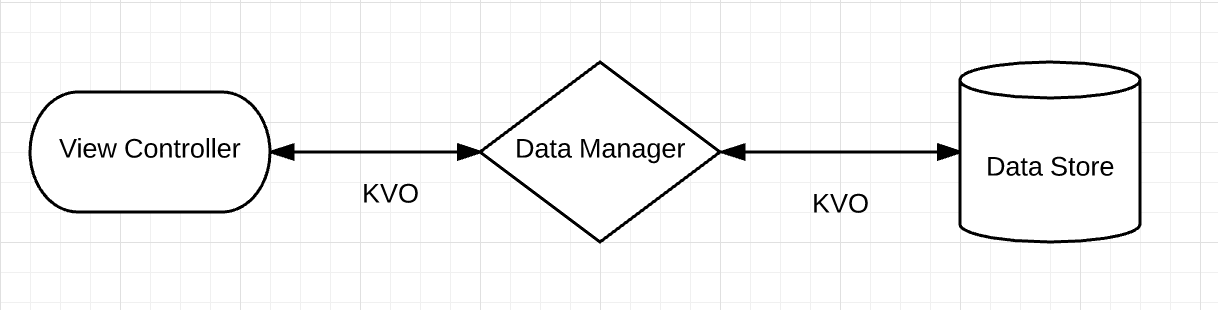
\includegraphics[width=\textwidth]{dataflow.png}

\section{Design Description Information Context}

\subsection{Introduction}
This section of the design document will provide information about the specific elements of design incorporated into the development of this application. Such areas include SDD identification, design stakeholders and their concerns, design views, design viewpoints, design elements, design overlays, design rationale, and design languages.

\subsection{SSD Identification}
This report is the initial SDD for the iOS Application in Swift project (C7FIT). The initial start date for this assignment was September 22, 2016. From there on out, we've been documenting design and specifications for our project C7FIT. As of currently, the design doc is not quite finalized yet The client of this project is eBay Inc., which is comprised of Luther Boorn, Splons Splonskowski, Wyatt Webb. The main objective of this design document is to illustrate the scope of the project C7FIT. The following sections will illustrate the concepts through visual diagrams.

\subsection{Design Stakeholders and Their Concerns}
The current stakeholders of the project are the clients at eBay Inc. including Luther Boorn, Splons Splonskowski, and Wyatt Webb. They are all developers and managers at eBay Inc. The main scope of the document is to layout the design of the C7FIT project. The main concerns in regards to this project is finishing the application on time with the current specifications. This document will utilize text descriptions as well as diagrams to portray the viewpoints of the project.

\subsection{Design Views}
This project is implemented through a MVC structure, which will allow for modular application development. Thus, adding new features and capabilities will be easily achievable. Because of the object oriented structure of the application, project development updates will be easily accomplished. Design views of the application will portray the user's schedule as well as user fitness data. The relationships between the varying MVC classes are easily defined. Dependencies render the the current facing challenges and potential future issues as well. Dynamic data displays the change of state between the various views in the application.

\subsection{Design Viewpoints}
Design viewpoints clearly display the expectations for interaction from the user in the application's various views. Dependency viewpoints display the various requirements of the system. Logical viewpoints portray the logical structure of the application. Interaction viewpoints render the interactions between the various classes of the application. These viewpoints are relevant to this project as the various states of the application encapsulate these fundamental components.

\subsection{Design Rationale}
Choices made for the design are decided accordingly with the specifications of the application's requirements. As the requirements shift and the client's evaluate the state of the application's development, the rational for the design may change as well. Each of the major design choices are commented on with relation to the rational behind each choice. This is done in order to allow for future developers to easily maintain the code base accordingly to the choices in design.

\subsection{Design Languages}
UML diagrams, Sketch designs, and user stories are utilized in order to layout the design of the application.

\section{Design Viewpoints}

\subsection{Introduction}
This section of the document will span various viewpoints for the application including context, composition, logical, dependency, information, pattern use, interface, structure, interaction, state dynamics, and resource viewpoints.



\subsection{Developing the User Interface}
To create the User interface, we will be coding the interface elements rather than using the drag and drop tools that come with Storyboards or Xibs. The custom code we have will be more complicated than the Storyboards or Xibs, but we can create custom stylings that are not possible with the other methods. The standard view layouts can be reused and repeated like a template. The code will make it hard to visualize our layout, however we will use the Storyboards to flesh out a prototype based off of the Sketches that we’ve created.

\subsubsection{Pattern Viewpoint}
From a patterning viewpoint, using code to develop our user interface will allow us to maintain a consistent pattern. This is because each viewing screen is self contained and can be replicated multiple times for different views. This replication gives us a consistent pattern between views. It makes it easier for the developer, as we don’t have to recreate the designs, and it makes the views consistent for the user. This makes the user interface more intuitive for the user.

\subsubsection{Context/User Viewpoint}
From the user’s viewpoint the popups created with code will be customized for each specific function. This will result in a better presentation, which will be more aesthetically pleasing for the app, and provide added functionality as Xib templates will not have exactly what we’re looking for. This means that we will be creating custom popups and views as shown by our Sketch Designs.

\subsubsection{Dependency Viewpoint}
The User interface will depend on the back end code of the application to perform actual functions. Likewise, the backend will depend on the user interface being developed for certain parts of the application to function. Controller elements that interact with the view, like selecting date/time or viewing trainer data will require that the view is created.



\subsection{Storing General User Data}
To store our general user data, we will be using CoreData to store local data on our application without the need of a backend database. CoreData is focused on storing objects with attributes rather than the more typical SQL tables. This allows it to have more flexibility in data storage at the cost of more overhead. We will be using CoreData to store data locally rather than having a server database, because the data stored will be relatively simple and will not require the large overhead of a remote server.

\subsubsection{Dependency Viewpoint}
All parts of the application that require the user to store data will be reliant on the local CoreData database to be set up. CoreData is natively supported by iOS so it will not be dependent on an external framework. The application’s daily youtube videos and quotes will not require CoreData because they will be stored and pulled from a GitHub page. The User’s personal record data, however, will require CoreData. They will store their PRs, such as push ups and mile times, locally on their device using CoreData. Additionally, the map tracking portion of the app will depend on a CoreData object to maintain information about the user’s activity path and time.

\subsubsection{Information Viewpoint}
Storing the data locally on the app rather than on a remote server allows the data to be entered in and accessed at any time without an internet connection. Much of the app requires the Firebase api to function, this is an unavoidable limitation as we don’t control the api; however, by storing user data locally the user will always have access to their information. This means that the information will persist whether or not there is an internet connection.

\subsubsection{User Viewpoint}
From the user’s viewpoint, storing the data locally benefits them because they will always be able to access the data. Like a note-taking application they will not be reliant on internet, and so they will be able to plan workouts on their own. Local storage allows the user to map and enter in their workout information conveniently when they don’t have internet. A use case would be when the user goes on runs in rural areas without wifi connectivity. This storage will still allow them to track their run information.

\subsubsection{Resource Viewpoint}
From a resource viewpoint, local storage puts a larger limitation on the application itself. If all of the user’s data is stored on the application they are limited to the size and power of their device. If they run out of space, then the application will be unable to store additional information. If we had used a remote server the user would not be dependent on the power of their device; However, we are limited financially to set up a server and consequently chose to be restricted by the device’s limitations. In normal conditions, the user will not be storing an excess amount of data that will overload the device’s capabilities.


\subsection{Choosing an IDE}
The IDE we will be using is XCode. XCode has all the built in support that we need for development using Swift 3, because the application is natively provided by Apple for development on iOS projects. This IDE is created and supported by Apple, and so it has extensive documentation. Additionally, it is the most popular IDE for the development of iOS applications so it has strong community support. It has a large amount of built in tools that allow the developer to simulate and debug their application without the need of the iOS device, although we will be testing both in the simulator and on our respective iOS devices (iPhone 5,6 and 7).

\subsubsection{Dependency Viewpoint}
The XCode IDE has the frameworks and technologies that we will need to develop the application already built in. As a design focus we have chosen a majority of native technologies like Swift 3 and CoreData, and so the native IDE will naturally support all of these choices. There is a device simulator built into the IDE so we can test the application on devices that we don’t own. On other IDE’s we would have to depend on XCode’s tools for this functionality as Apple limits much of their tools to their own software.

\subsubsection{Resource Viewpoint}
From a resource viewpoint, using the XCode IDE costs the team nothing. It provides some of the best functionality available for an iOS IDE, and is offered for free on Apple’s computers. The functionality from the IDE gives the team powerful tools without any resource expenditure.

\subsection{Parsing Firebase Data}
Most of our app is built around the Firebase service. Firebase is a software suite that helps gyms, studios, and other wellness centers run their business. It manages responsibilities such as handling membership / service payments, scheduling appointments, tracking customer metrics, and more. Most of this functionality is accessible via a SOAP XML API, a type of web-based protocol to communicate with an external service.\\

Since SOAP XML API’s are considered obsolete, and have been mostly replaced with JSON-based API’s, there is little innovation in XML parsers, especially on newer platforms such as iOS. However, in the early 2000’s, SOAP was the norm and there are therefore several performant and stable options available for our use. The only issue is that none of these parsers were written with a Swift API, so we will therefore need to write a wrapper around the libraries we choose. We have decided to use Apple's XMLParser library for this purpose

\subsubsection{Logical Viewpoint}
Our wrapper will consist of a functional interface that will simply convert NSData XML objects received from the API into Swift structures or classes. The functions we use to do this will know the structure of the Firebase API responses and will use the XMLParser library to parse them.

\subsubsection{Dependency Viewpoint}
Our parsing library for Firebase will be a wrapper for Apple's XMLParser library. This library is a 1st party dependency, as it is built into Apple's Foundation framework available to every iOS app.

\subsubsection{Algorithm Viewpoint}
Some data structures received from Firebase may be nested inside other data structures. To parse a parent data structure with children data structures, we will use recursive programming - parsing the children before moving up into the parent data structure. This decision is partially guided by Swift's strict type system, which would require a parent structure's children to be of a Swift object or struct type, instead of a raw data type.

\subsubsection{Patterns Viewpoint}
When creating these functions, we may find it useful to create convenience parsers to parse different kinds of input. Instead of rewriting the logic of every function just to take different type parameters, we should use composition - creating a base function that all convenience functions will use underneath. Therefore, convenience parsing functions will only have to perform a type conversion for their parameter into the parameter required by the base function. The base function's input parameter should either use the most primitive type available, such as a string, or the input parameter required by the XMLParser library.


\subsection{Handling Touch Events}
Touch is the primary source of user interaction with iOS applications and handling touch events is likely the most important aspect of any app. In our opinion, the most important attributes of good touch handling are:

1. Correctly and swiftly determining intentional touch events, while filtering “noise”.\\
2. Correctly placing touch events on the screen. According to interviews with high-level Apple engineers\cite{touchpara1}, this is not just a case of being accurate — where users actually touch the screen is a different location than where they expect to see the touch registered.\\
3. Providing a simple API that hides superfluous details.\\

Apple’s UIKit framework contains several UI elements (buttons, sliders, labels, etc), and most of these have gesture/touch-recognition built in. For elements that don’t have built in gesture recognition, UIKit provides a UIGestureRecognizer class which can be easily overlaid on an element’s view area.
We have decided to use UIKit's elements exclusively unless it is absolutely necessary to build a custom component or to add touch handling to a existing UIKit component that lacks it.

\subsubsection{Composition Viewpoint}
Since touch is such a large part of iOS, Apple has the design patterns pretty hammered out. If we want to observe an element designed in a XIB file (graphical user interface designer), we can drag a touch handler from the the XIB file to our code. This touch handler is a function that is called whenever the element is touched. We can then filter out the undesired touch events using a switch statement to appropriately respond to taps, drags, zooms, and more. \\

In the event the element we want to observe is dynamically added to the screen or otherwise not in the XIB file, it is possible to handle touches by calling: \begin{lstlisting}
addTarget(_:action:for:)
\end{lstlisting}
this method is called on a child of the UIResponder class and allows us to specify a target class and method to be called for a specified gesture.

\subsection{Storing/Modifying Application State}
Apple's frameworks provide a lot of functionality, but do little to tell developers how to manage their application's state. They are opinionated however, and they provide some components such as storyboards that make creating a simple app easy, but can become convoluted as an app grows. Since our app is relatively complicated, we want to remember to think big when designing how our application manages its state.\\

We have decided to opt for using a central data store in our application that is passed to each view controller via dependency injection. This solves a host of problems, including reducing data fragmentation, easing persistence, reducing confusion, and more. It also creates some cool benefits, such as making it easy to track and roll back app state, making it a lot easier to debug issues.

\subsubsection{State dynamics}
While it would be unreasonably difficult to design our entire state machine before implementing the app, we will try to outline the main components and behavior of the data store below. \\

When the app is launched for the first time, it will have no data from the Firebase service to display. While subsequent launches will likely have some cached data to display, it is useful to first consider the initial state. Much of the information displayed will be in arrays of Swift classes or structures. To force the views to consider the null state, we will code these arrays as optionals (can be null). Once data is received from the API, the arrays will be initialized and filled with data. In the case of no data being received, the array could either stay null or be initialized with zero elements. We will likely utilize both methods, along with the use of exceptions to display useful information to the user at all times. \\

The datastore is mostly intended to handle the app's data state, but it would be interesting to also put view state inside either the central datastore or a additional datastore. This would allow us to easily fully restore the app's previous state. Likely this would just entail creating an enumeration that reflects the app's navigation stack of view controllers.

\subsection{General}

\subsubsection{Context Viewpoint}
The primary users of the C7FIT application will be members of the Club Seven Gym in Portland, Oregon. Club Seven, run by owner Brian Warner, is a small, personal training-focused gym that works closely with its members to achieve their individual goals. The gym also works with atheletes, especially student atheletes, and has hired an ex-OSU football player Sylvester Green to coach clients.

As a small gym, the owner likely doesn't have a full-time staff to answer phones, manage payments, and schedule training sessions. Luckily, these processes can be handled by the Firebase platform, which the gym uses to manage these tasks. While Firebase provides a customizable client-facing web portal for gyms, it doesn't have any client-facing applications for scheduling, paying, viewing gym info, etc. This is mostly due to the fact that it is logistically difficult for a company such as Firebase to release and maintain individual apps for each of its partner gyms. The Apple App Store makes it tedious to release app updates, and keeping every version of a Firebase app up to date would be difficult, if not outright banned by Apple.

If a specific gym wants a mobile app, they need to build one themselves, which we are doing for Club Seven.

\subsubsection{Patterns Use Viewpoint}
For this project, we will enforce a strict pattern for our data flow to ensure we always know where our data is stored. We will use the Dependency Injection pattern to enforce this, creating a single datastore object during our app's instantiation. As new views are presented, the root view controller should inject a reference to this datastore object into the new presenting view controller. \\

There are several advantages to this approach. First, since view controllers will require the datastore in their initializer, their datasource will be explicitly defined and it will be impossible to instantiate a view withiout it having valid data to display. Second, since all views share the same data source, they will not need to needlessly copy data for themselves. Thirdly, since all views will share the same data source passed in from their parent, there will not be inter-dependencies between views. This will result a tree-like data flow instead of the web-like data flow that develops in many large and poorly-designed applications. Finally, the app's full state will be shared among all views in the app, eliminating fragmentation as long as views are kept up-to-date with the datastore. This leads us to our second major design pattern, reactive programming. \\

There is another pattern that goes along well with this central datastore approach called functional reactive programming. Functional reactive programming consists of composing a series of pure functions that watches an underlying data source. When the data source changes, the functions run and transform the underlying data from one form to another. We intend to use reactive programming to ensure our views stay up to date with our app's state. This will be accomplished by binding view elements to the datasource, with functions in-between to convert the data source's data into a presentable view object. Whenever our data changes, the parts of the view that should be updated should then "react" without requiring additional code. This helps eliminate a lot of mistakes with writing "update" functions. Often these functions don't update the correct parts of view, update too much of the view, or cause unexpected side-effects.

\subsubsection{Interface Viewpoint}
Client side user interface is important to any application. Rendering a consistent and elegant design for the user to interface with is vital to the user experience. Below are a few Sketch designs for the various potential views in C7FIT.

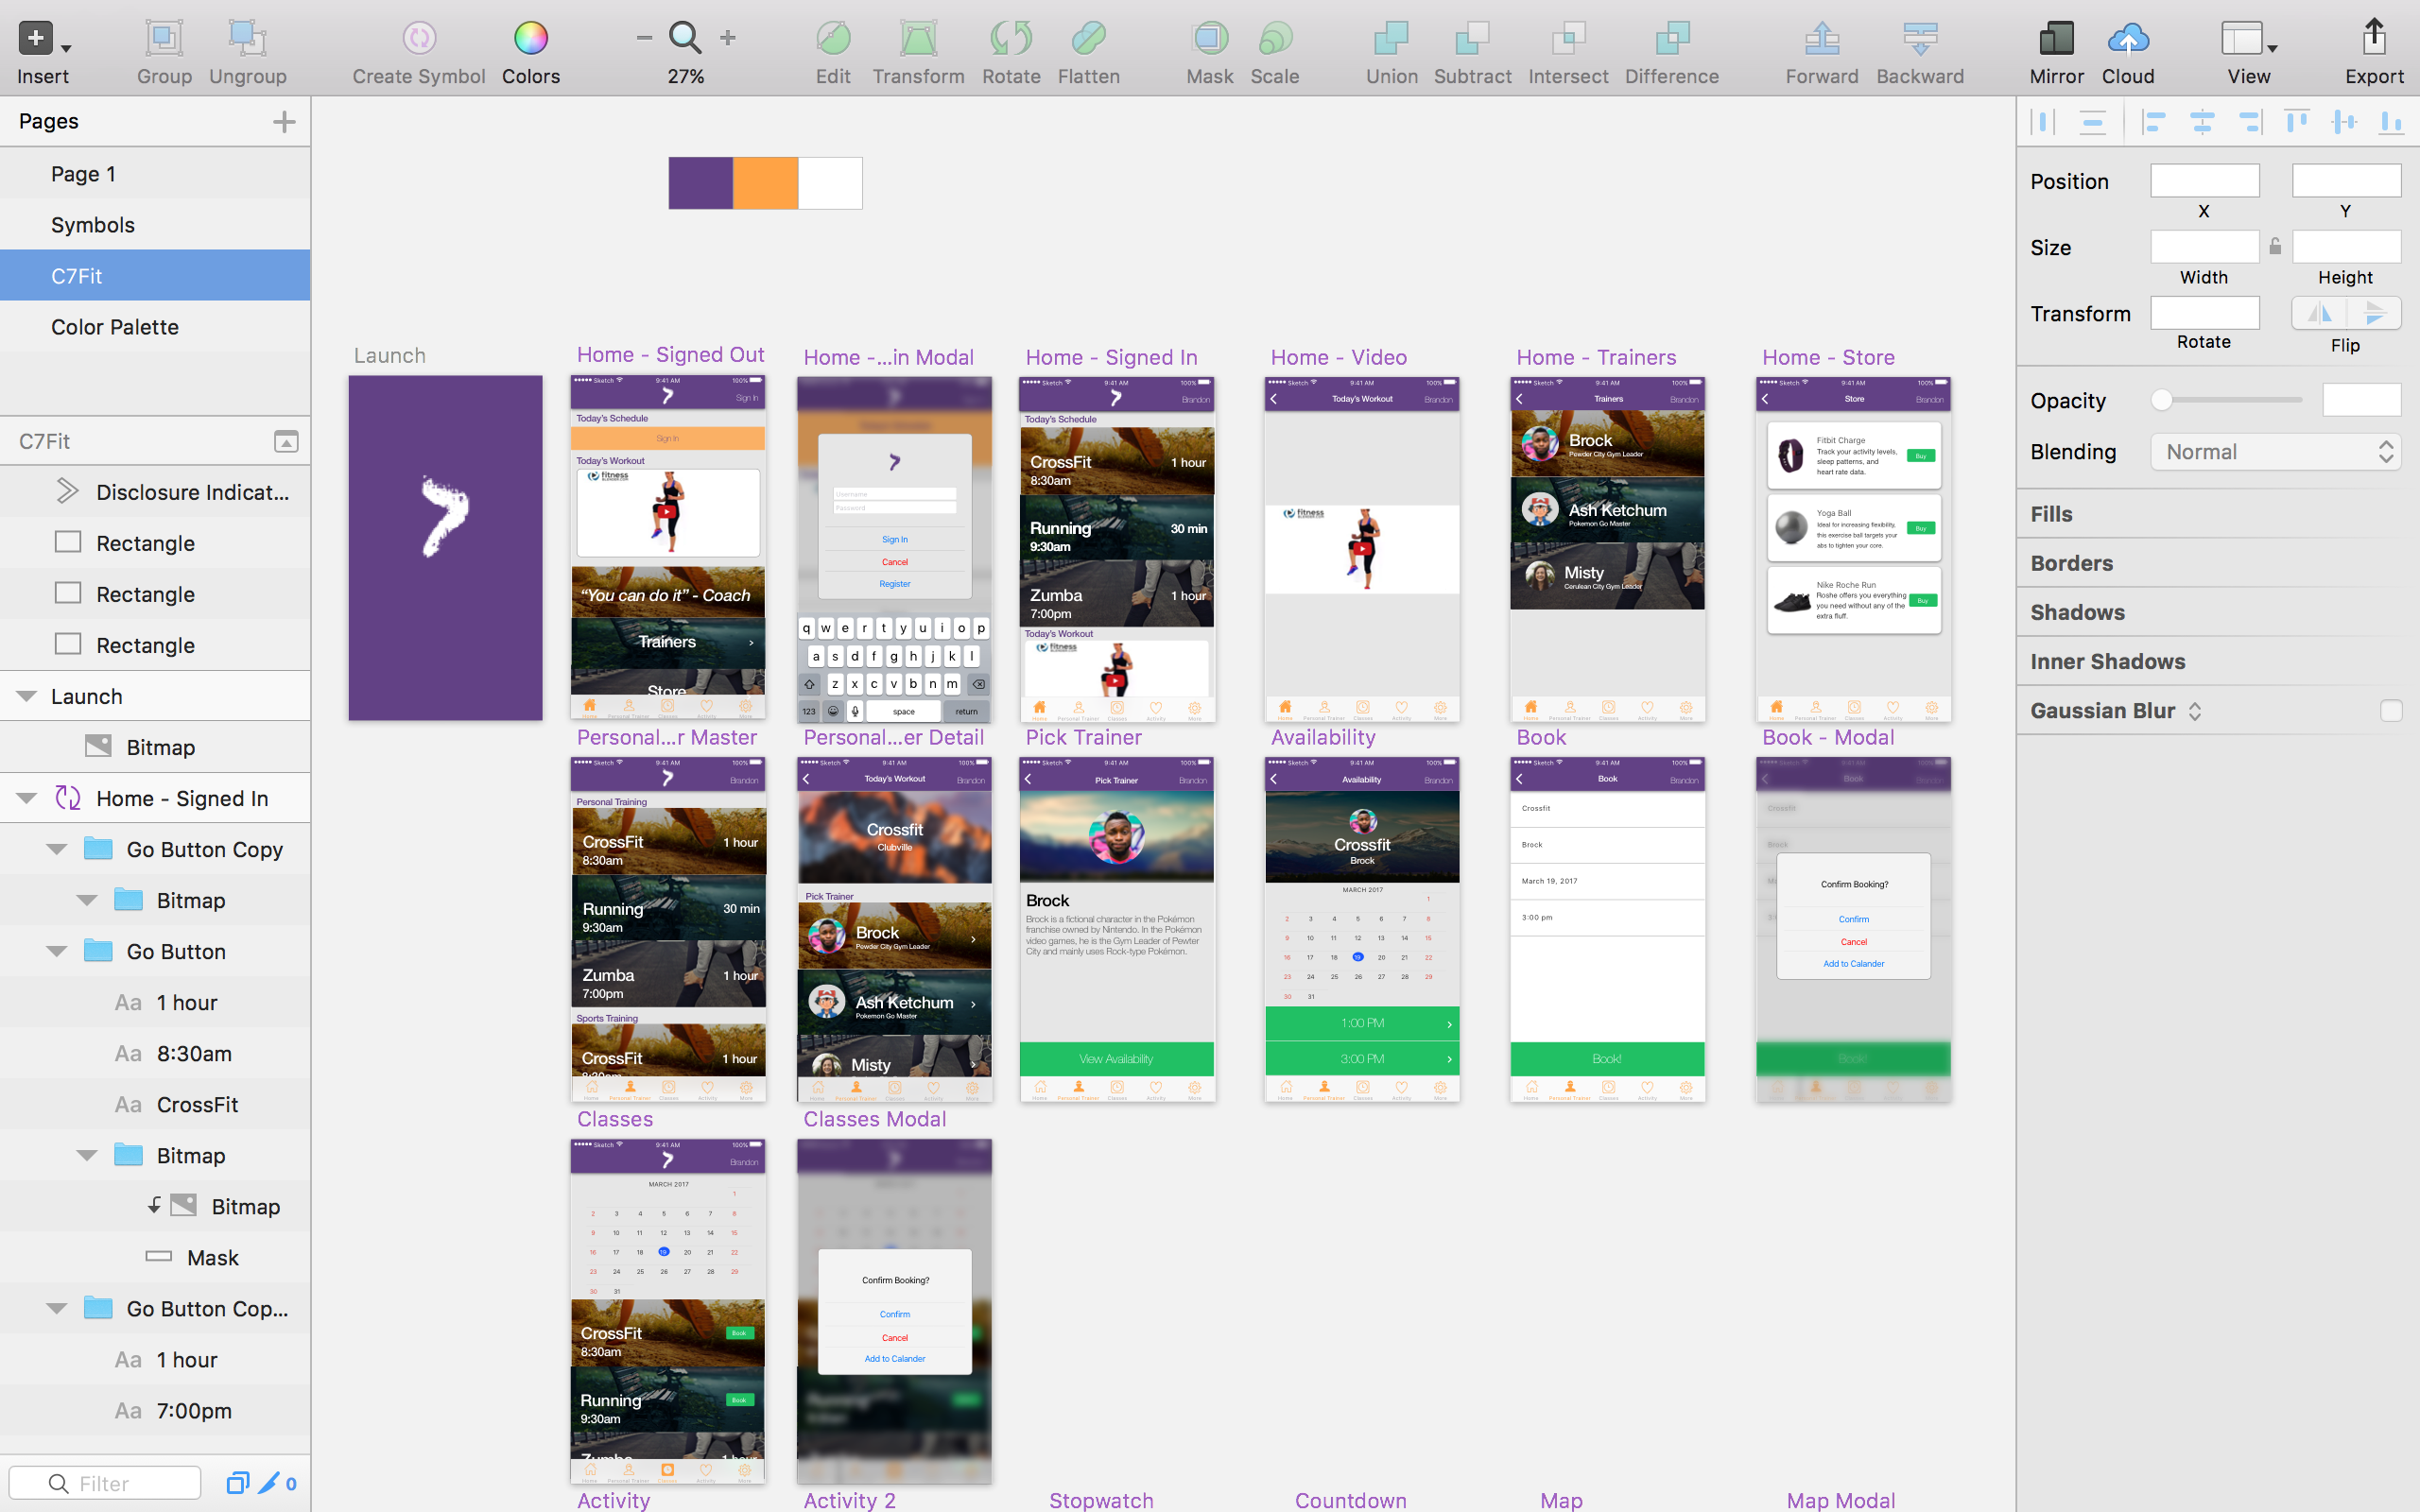
\includegraphics[width=\textwidth]{sketch1.png}\\
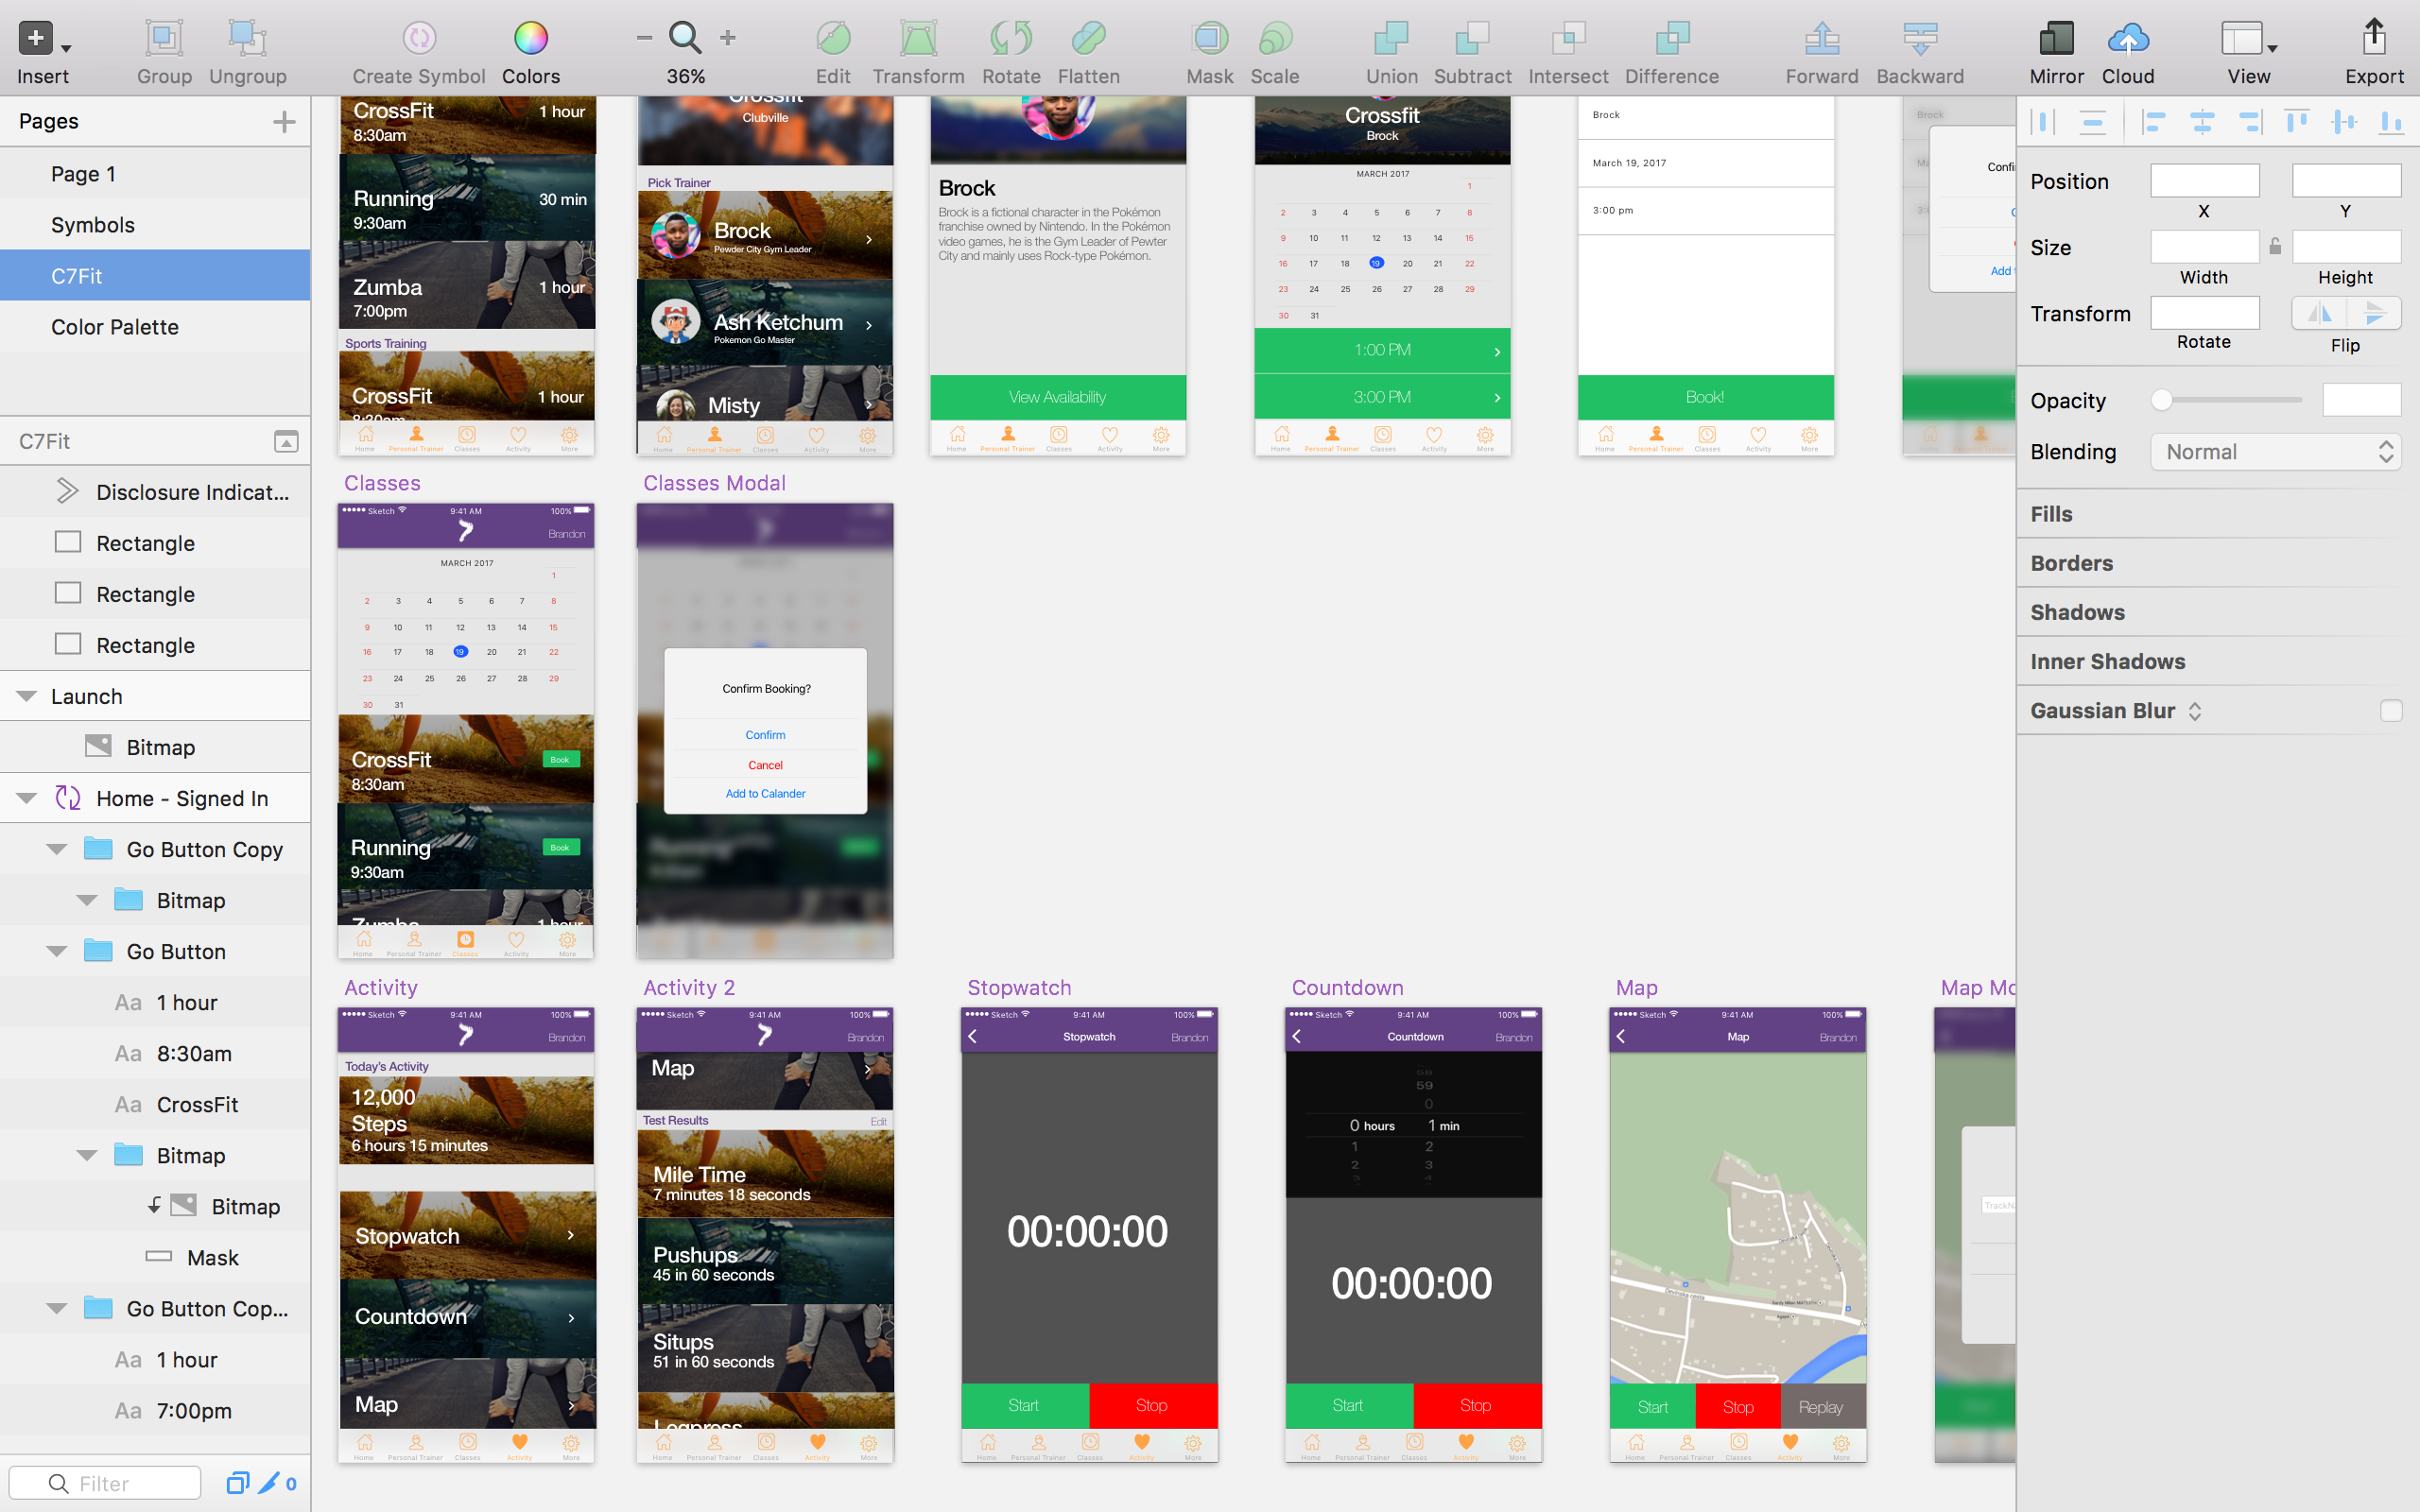
\includegraphics[width=\textwidth]{sketch2.png}\\
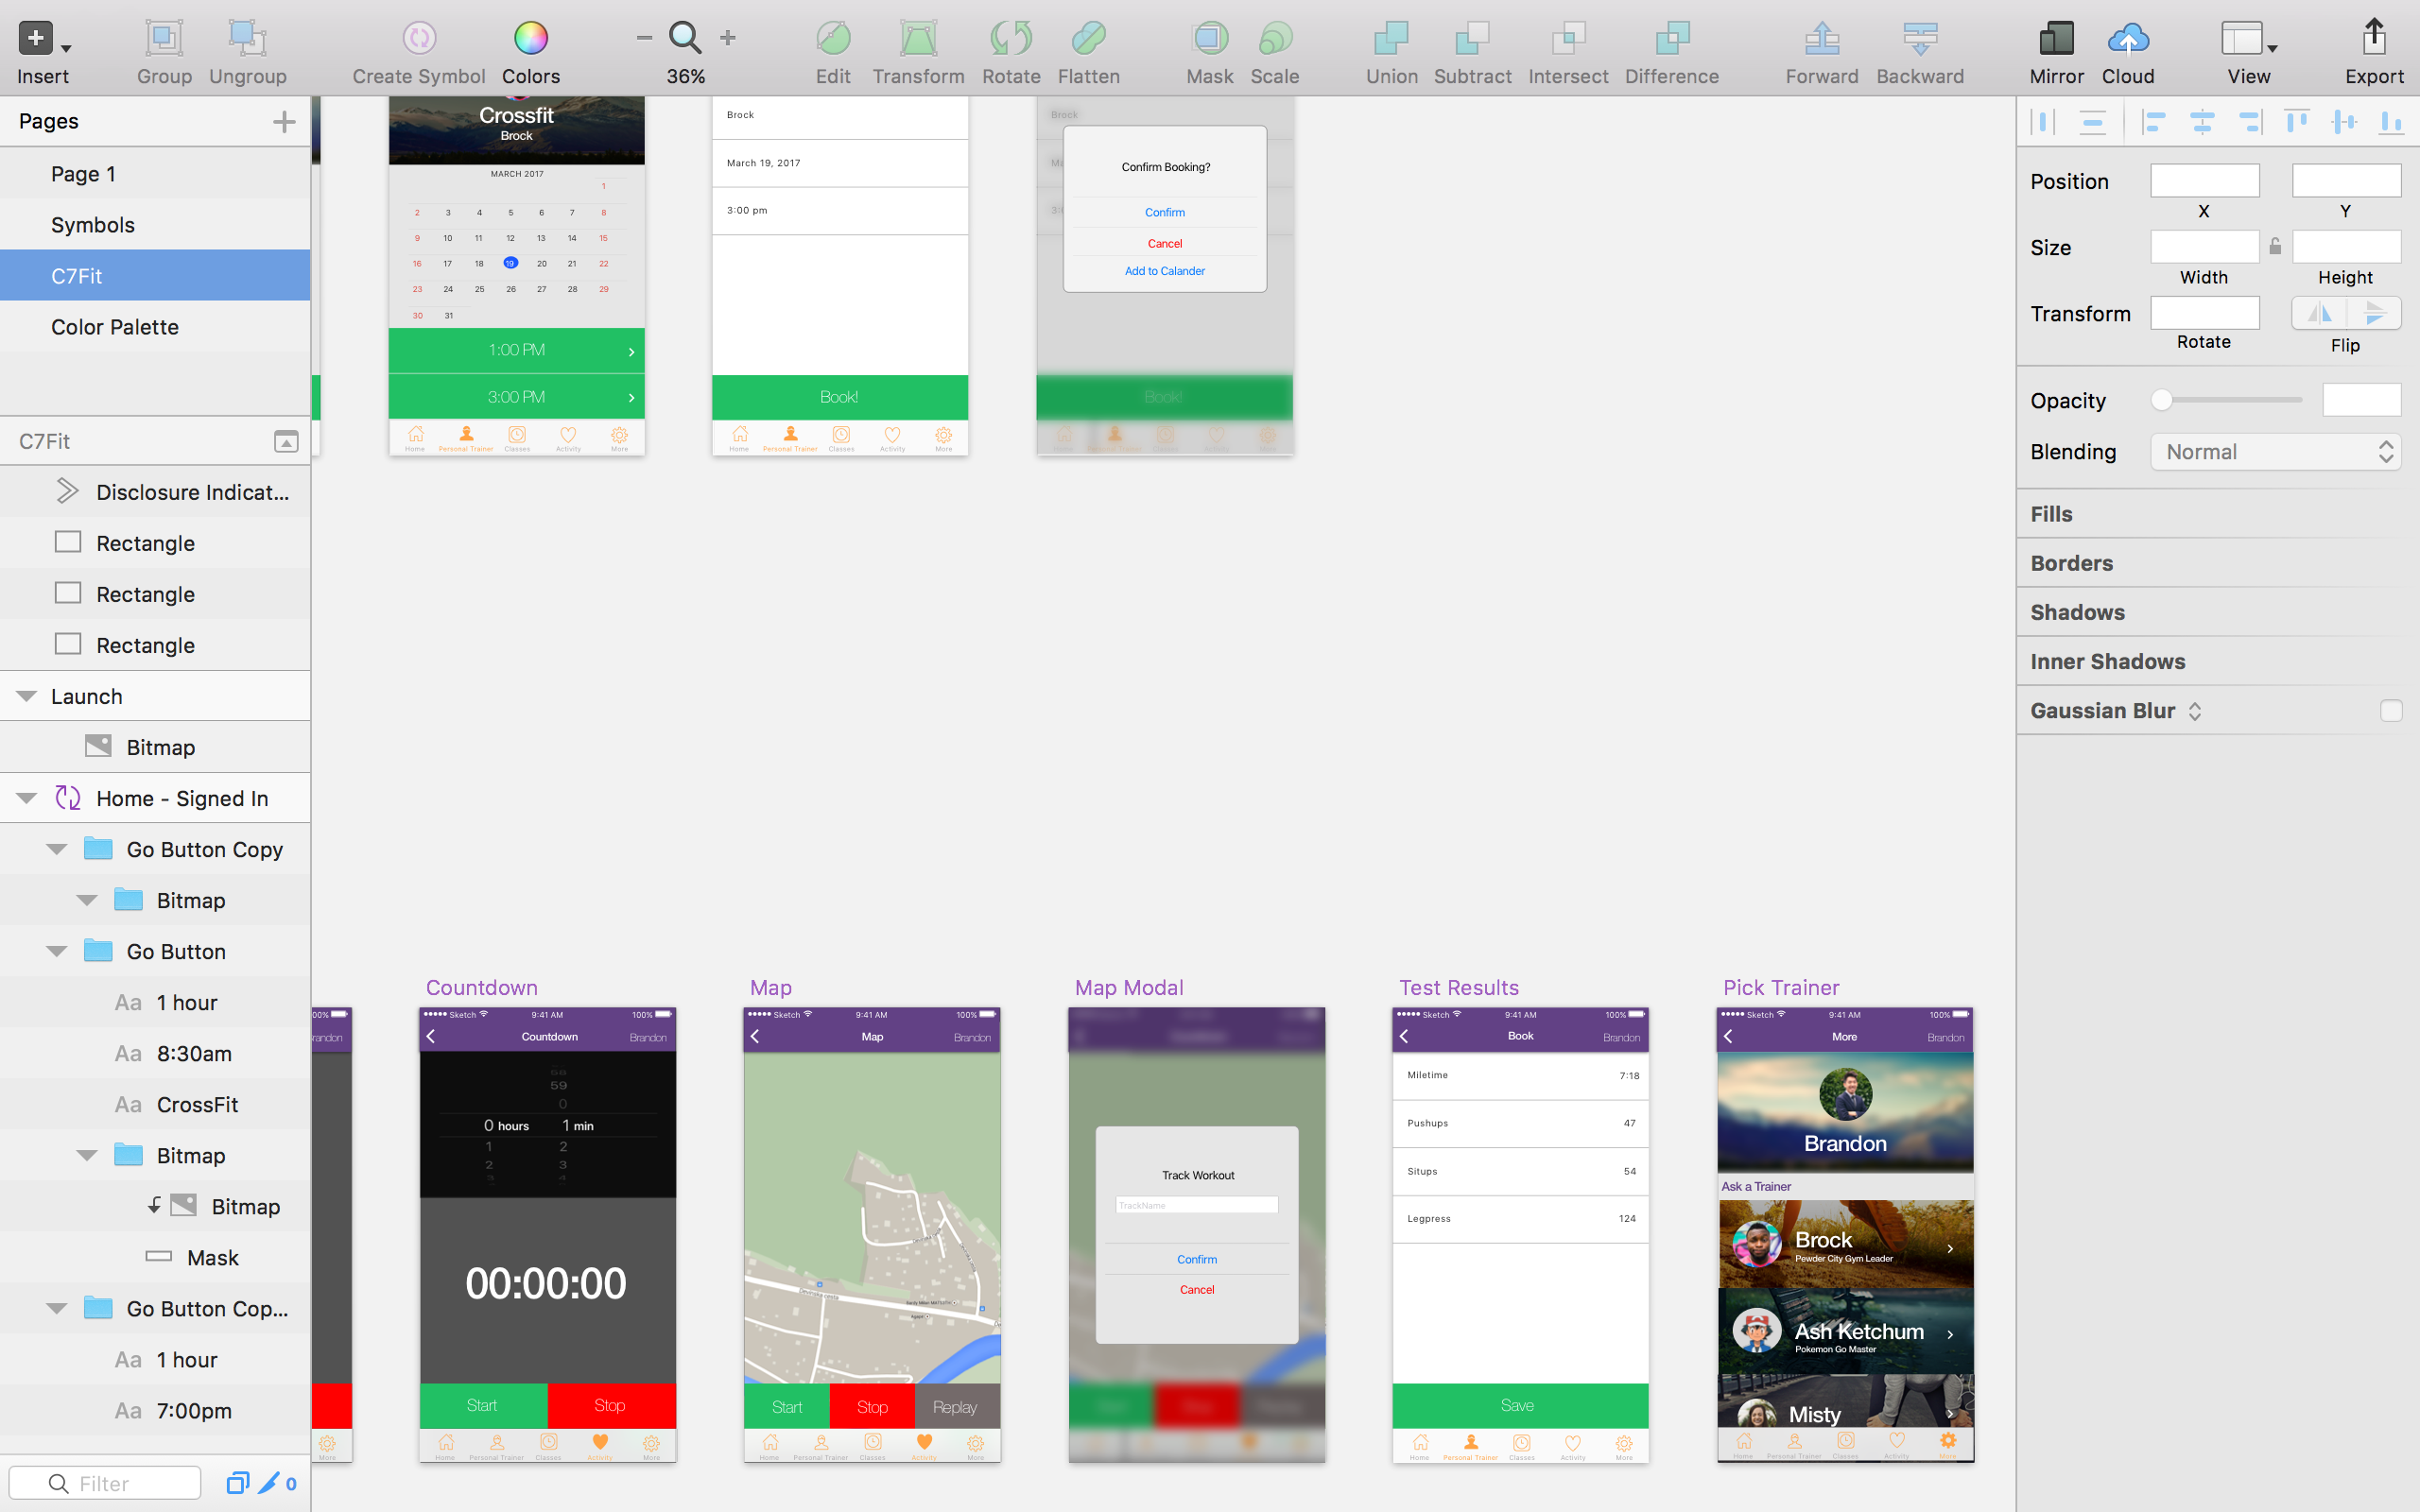
\includegraphics[width=\textwidth]{sketch3.png}\\

\section{Conclusion}
The designs in this document were evaluated on different criteria, some of the more important criteria being native availability, functionality, and visual-ability. We wanted designs to be simple to understand, and at the same time to portray a clear message on what our intentions are. Many of our designs were driven for iOS.\\


\newpage

\section{Signed Participants}

\textbf{Students}

Brandon Lee\\
Rutger Farry\\
Michael Lee\\

\end{document}
